\chapter{Descrizione della zona in esame e degli eventi studiati}

\section{Sismicità e tettonica della Kamchatka}
La penisola della Kamchatka è una regione della Russia orientale situata nel nord-ovest del Pacifico, lunga \qty{1250}{\kilo\meter} (\(51-61^\circ \text{N}\)) e larga \qty{450}{\kilo\meter} (\(155-163 ^\circ \text{E}\)) \citep{glacier_mass}. Questa zona è tra le più sismicamente attive del pianeta. Infatti, dall'inizio del secolo scorso sono stati registrati diversi grandi terremoti, inclusi sei eventi con magnitudo superiore a 8: nel 1904 (\(\mathrm{M}\,8.0\)), 1923 (\(\mathrm{M}\,8.5\)), 1952 (\(\mathrm{M}\,9.0\)), 1959 (\(\mathrm{M}\,8.2\)), 1997 (\(\mathrm{M}\,7.8\)) e nel 2025 (\(\mathrm{M}\,8.8\)). In particolare il terremoto del 1952 è il quinto terremoto più potente che sia mai stato registrato.

Questa regione fa parte dell'arco delle Curili-Kamchatka, che si estende per circa \qty{2100}{\kilo\meter}, partendo da Hokkaido in Giappone, passando per le isole Curili e la penisola della Kamchatka, terminando intersecandosi con l'arco delle isole Aleutine, a sud delle isole del Commodoro in Russia.
L'arco delle Curili-Kamchatka si è formato in corrispondenza della zona in cui la placca del Pacifico subduce nel mantello sotto la micro-placca di Okhotsk, considerata una suddivisione della placca Nordamericana \citep{usgs2025qw60}. La subduzione avviene con un rate di \(77~\mathrm{mm/yr}\) vicino alla parte settentrionale dell'arco (\(55 ^\circ \text{N}\)) fino a \(83~\mathrm{mm/yr}\) nella zona prossima ad Hokkaido (\(47 ^\circ \text{N}\)) \citep{description}.

Studiando la struttura litosferica lungo la costa orientale della Kamchatka è stato stimato che la crosta abbia uno spessore tra i \qty{30}{\kilo\meter} e i \qty{40}{\kilo\meter}, tramite misure di gravità e rilevazioni sismiche a sorgente attiva \citep{bogdanov2000tectonic} e modelli di funzioni di ricevitore teleseismiche \citep{levin2002}.
Tali spessori sono comparabili alla profondità dei terremoti generati da faglie di sovrascorrimento lungo la placca subdotta, evidenziando il legame tra struttura litosferica e sismicità nella regione.
L'arco delle Curili-Kamchatka è infatti una delle aree più sismicamente attive al mondo: la deformazione della placca Nordamericana sovrastante genera terremoti crostali poco profondi, mentre lo scorrimento lungo il piano di subduzione tra la placca Pacifica e quella Nordamericana produce terremoti che si estendono fino a profondità di 40-60 km \citep{usgs2025qw60}.

La morfologia della placca del Pacifico cambia a \(53.5-54.5 ^\circ \text{N}\), quando questa incontra il monte sottomarino Meiji (Meiji Seamount), cambiando il carattere della subduzione. L'angolo di subduzione decresce da sud a nord da \(55 ^\circ\) a \(35 ^\circ\) e la massima profondità della sismicità si riduce da \(\sim\) \qty{600}{\kilo\meter} a \(\sim\) \qty{200}{\kilo\meter}, provocando una deviazione verso nord-ovest del fronte vulcanico \citep{description, usgs2025qw60}.


\section{Terremoto M8.8 del 29/07/2025}

Il 29 luglio 2025 (30 luglio alle 11:24 ora locale) si è verificato un terremoto \(\mathrm{M}\,8.8\) nel sud della Kamchatka, tra i 10 più potenti mai registrati, prodotto dalla stessa zona di subduzione che generò nel 1952 un terremoto \(\mathrm{M}\,9.0\).
L'epicentro dell'evento è stato localizzato alle coordinate \(52.495^\circ \text{N}\) e \(160.240^\circ \text{E}\), ad una profondità di \qty{35 +- 1.8}{\kilo\meter} \citep{usgs2025qw60}.
Terremoti di questa magnitudo si verificano in prossimità di zone di subduzione e sono generati da una faglia detta di \textit{megathrust} (di mega-sovrascorrimento). Le faglie megathrust sono faglie inverse di grandi dimensioni, situate solitamente lungo margini convergenti. Per quanto riguarda la Kamchatka, la faglia separa la placca del Pacifico che subduce a quella Nordamericana \citep{hubbardstrikeskamchatka}. 

Terremoti di questa portata sono eventi piuttosto rari. In un loro articolo, \citet{hubbardfirstlook} prendono in considerazione i diciassette terremoti di magnitudo \(\mathrm{M}\ge 8.5\) avvenuti dal 1900 ad oggi. La loro analisi prosegue cercando una dipendenza tra questi eventi e i \textit{foreshock}, terremoti di minore entità che ne precedono uno maggiore, in particolare ricercando la correlazione tra foreshock di magnitudo \(\mathrm{M} \ge 7\) e gli eventi di magnitudo  \(\mathrm{M} \ge 8.5\).
Ne risulta però che la correlazione è di \(\sim1 \%\), mostrando che questi eventi sono difficili da prevedere attraverso l'analisi dei foreshock. 
Terremoti di questo tipo, proprio per la loro sporadicità, sono un importante oggetto di ricerca.

L'ente statunitense United States Geological Survey (USGS) si è occupato da subito dello studio del terremoto, calcolando gli spostamenti prodotti e il momento sismico tramite un modello \textit{finite fault} (a faglia finita) \citep{usgs2025qw60finitefault}.
Modelli di questo tipo utilizzano dati riguardanti il movimento del suolo causato dal terremoto (come lo studio di onde sismiche rilevate da stazioni sismografiche e di spostamenti della superficie terrestre) riuscendo  a rappresentare la dimensione della faglia e l'intensità dello slip lungo di essa \citep{usgs_finite_fault}. Un approccio di questo tipo, in cui si studiano gli effetti per arrivare alla causa è detto problema inverso. Tipicamente, un piano di faglia viene diviso in numerose subfaglie di dimensioni minori e tramite il problema inverso si riesce a stabilire lo slip subito da ognuna di esse, andando a ricostruire il comportamento totale della faglia.

\begin{figure}[!b]
    \centering
    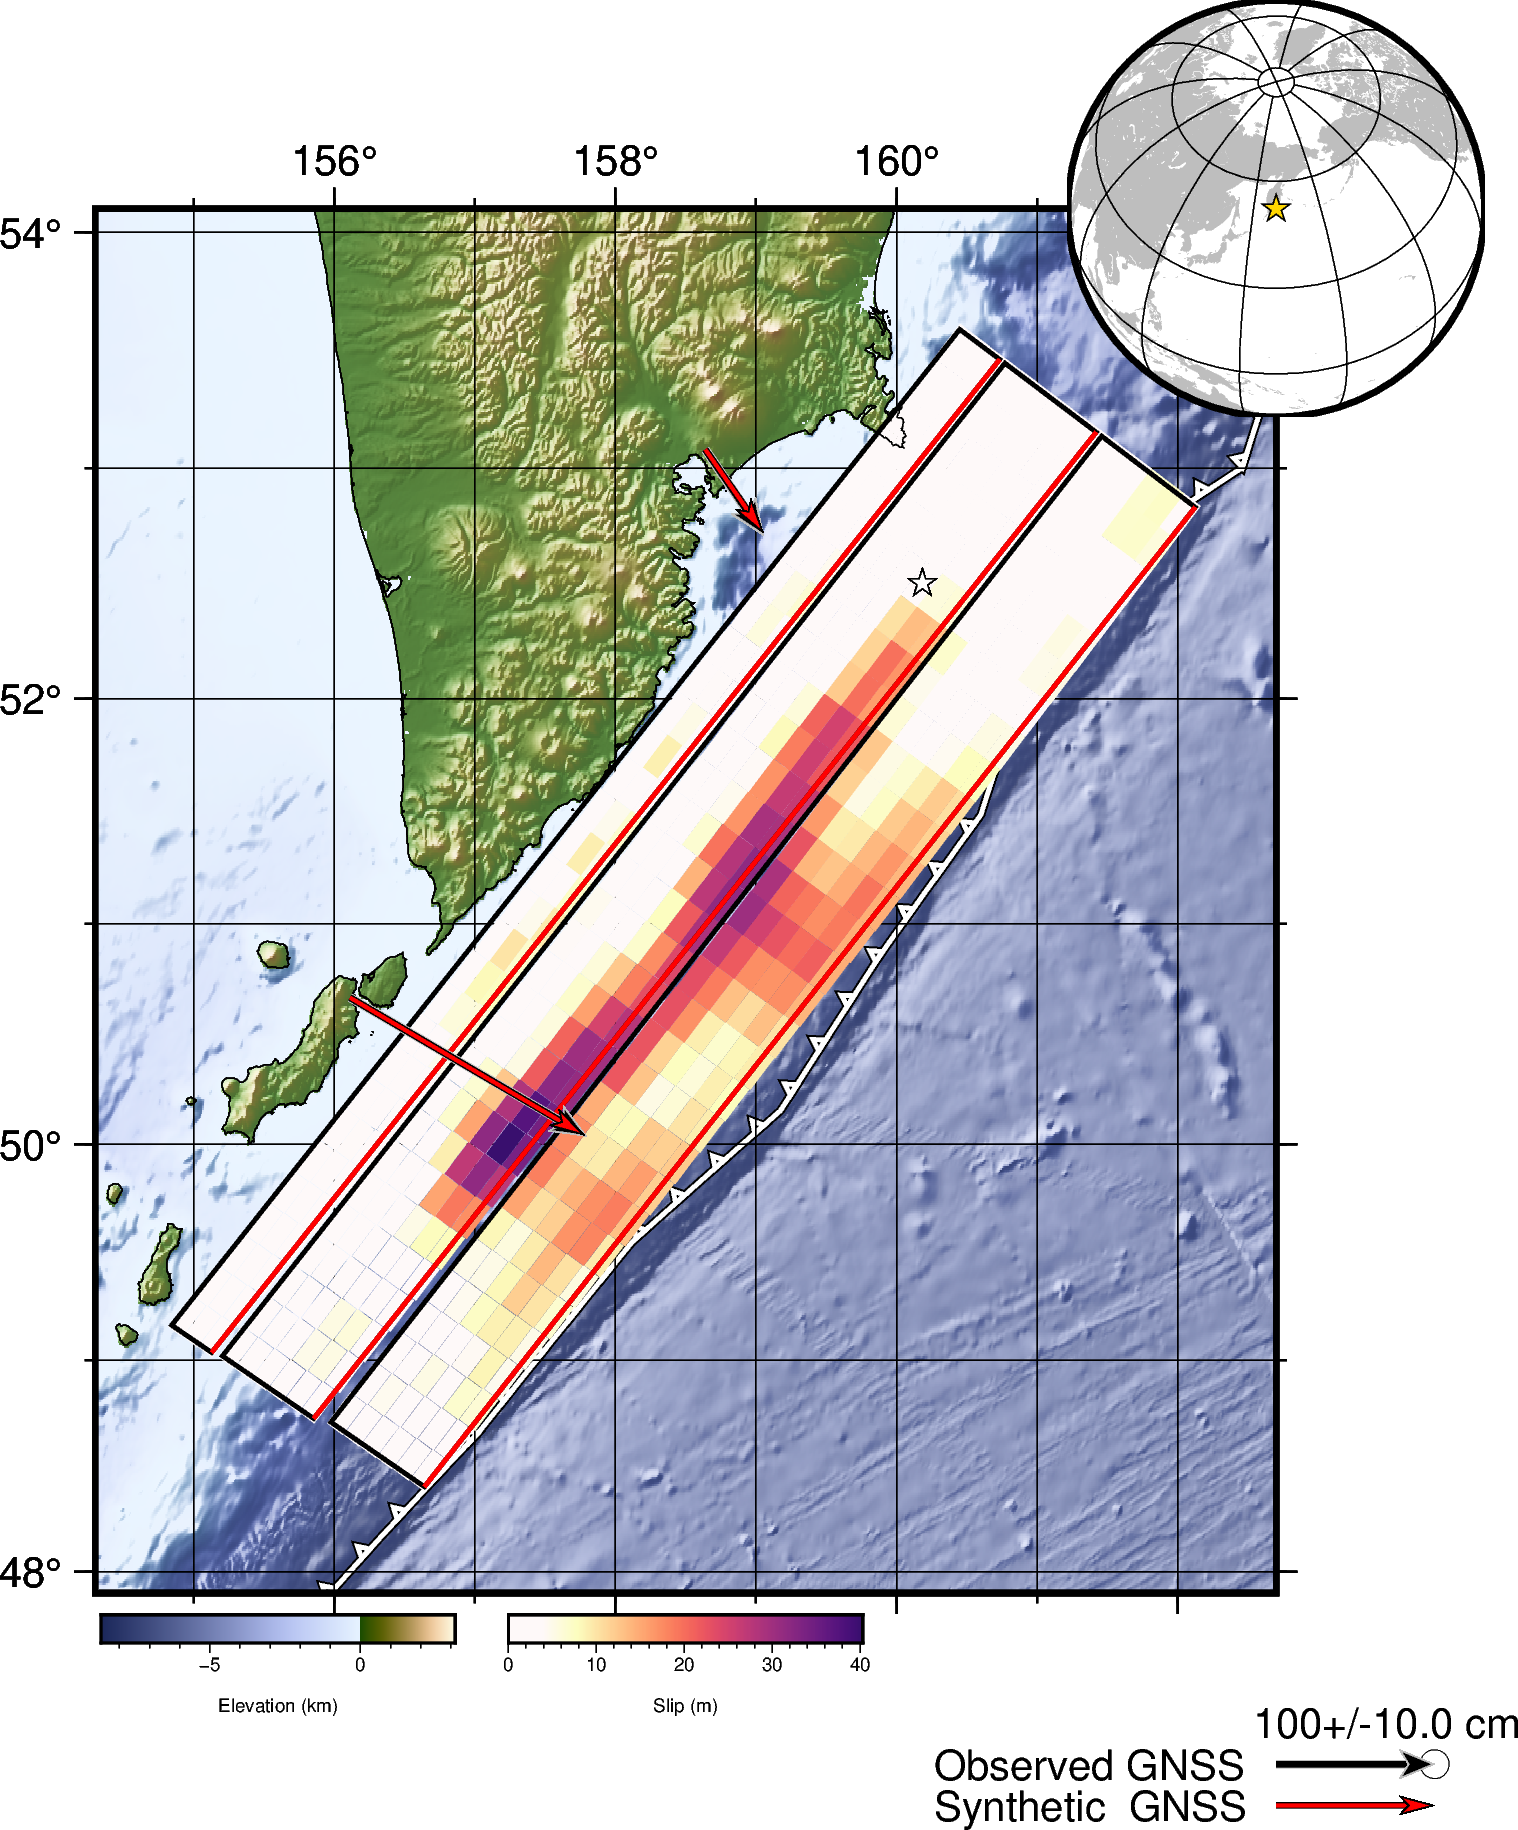
\includegraphics[width=0.7\linewidth]{graphics/basemap.png}
    \caption{Proiezione superficiale dello slip per il terremoto del 29 luglio 2025 in Kamchatka. La scala di colore dal bianco al blu indica l'intensità dello slip. La linea bianca indica il confine tra due placche [preso da \citep{usgs2025qw60finitefault}].}
    \label{fig:basemap}
\end{figure}

Nell'analisi del terremoto in questione il USGS ha analizzato onde sismiche raccolte da stazioni sismografiche situate in tutto il mondo e ha aggiornato il modello nelle settimane seguenti. Il primo miglioramento del modello è stato realizzato andando ad implementare dati provenienti da radar satellitari, raccolti utilizzando il metodo inSAR (Interferometric Synthetic Aperture Radar) \citep{hubbard2025kamchatkaupdates}. Questo metodo consiste nell'utilizzo di onde radio o microonde a una specifica lunghezza d'onda inviate da un satellite sulla superficie terrestre. Diversi punti della superficie riflettono le onde con una fase diversa, che può essere ricavata misurando l'ampiezza dell'onda e può essere rappresentata tramite una mappa di fase. Poiché un terremoto è un evento in grado di andare a modificare la superficie terrestre, è possibile realizzare un interferogramma tramite due immagini ottenute dal satellite, una prima e una dopo l'evento sismico, per studiare così gli spostamenti avvenuti \citep{hubbard2023inSAR}.

Un'ulteriore miglioramento nel modello è stato fatto andando a considerare che la geometria della faglia è quella di una superficie curva e non piana. Per questo motivo il piano della faglia è stato suddiviso in tre segmenti con diverso dip (angolo di immersione). Questo è più piccolo lungo la faglia e cresce in direzione nord-ovest \citep{hubbard2025aftershockupdate}.
Nello specifico, in Fig. \ref{fig:basemap} viene mostrata una proiezione della distribuzione superficiale dello slip. Il valore massimo raggiunto dallo slip è di \( \sim\) \qty{40}{\meter}. In generale risulta abbastanza contenuto tra la costa e la faglia, senza raggiungere la penisola.


\section{Attività vulcanica in Kamchatka}
I vulcani sulla superficie terrestre non sono distribuiti casualmente. La maggior parte di questi si trova ai margini dei continenti, lungo catene di isole, o sotto il livello del mare dove formano lunghe catene montuose. In particolare, più della metà dei vulcani attivi si trova nell'oceano Pacifico \citep{usgs_volcanoes_plate_tectonics_1997} e forma quella che viene chiamata ``Cintura di Fuoco", che circonda il Pacifico passando proprio per la Kamchatka (Fig. \ref{fig:fire_ring}).
Si nota, infatti, come la formazione di catene vulcaniche avvenga principalmente lungo i confini delle placche tettoniche.

\begin{figure}[!t]
    \centering
    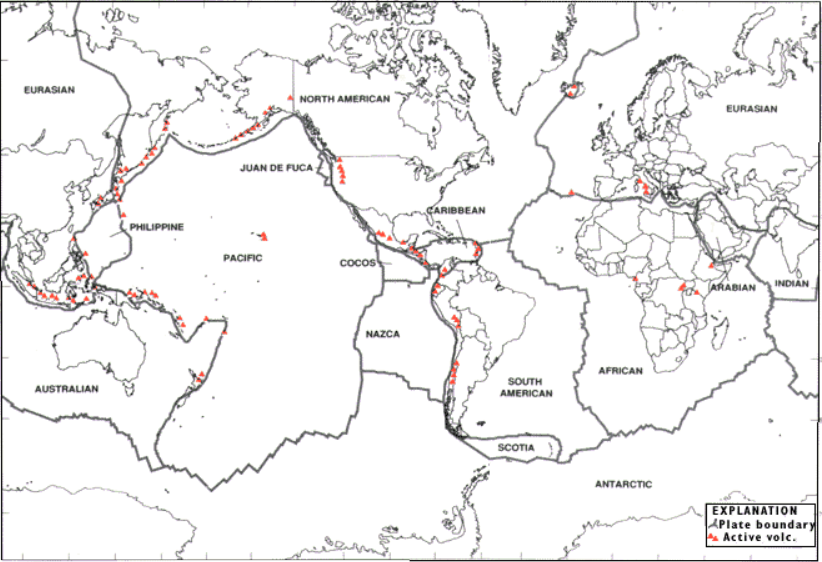
\includegraphics[width=0.7\linewidth]{graphics/fire_ring.png}
    \caption{Mappa indicante i confini delle placche e la posizione di diversi vulcani in attività nella Cintura di Fuoco nel Pacifico. I margini divergenti sono indicati tramite linee doppie, quelli convergenti con linee dentate. Gli archi vulcanici si trovano nella zona evidenziata in rosa, rappresentati attraverso linee magenta [preso da \citet{Britannica2025}]}
    \label{fig:fire_ring}
\end{figure}

La penisola della Kamchatka è tra le regioni con la più alta attività vulcanica del pianeta; attiva da più di 70 milioni di anni (\qty{}{Ma}) \citep{volcan_kam} a causa della subduzione della litosfera oceanica della placca del Pacifico sotto la micro-placca di Okhotsk.

Grazie al processo di subduzione, la placca del Pacifico, immersa ad elevate profondità, rilascia componenti volatili che producono un abbassamento nella temperatura di fusione del mantello. Alla profondità di circa \qty{100}{\kilo\meter} \citep{Shu2022Kamchatka} si ha quindi produzione di magma (Fig. \ref{fig:subduzione_kamchatka}).
\begin{figure}[t]
    \centering
    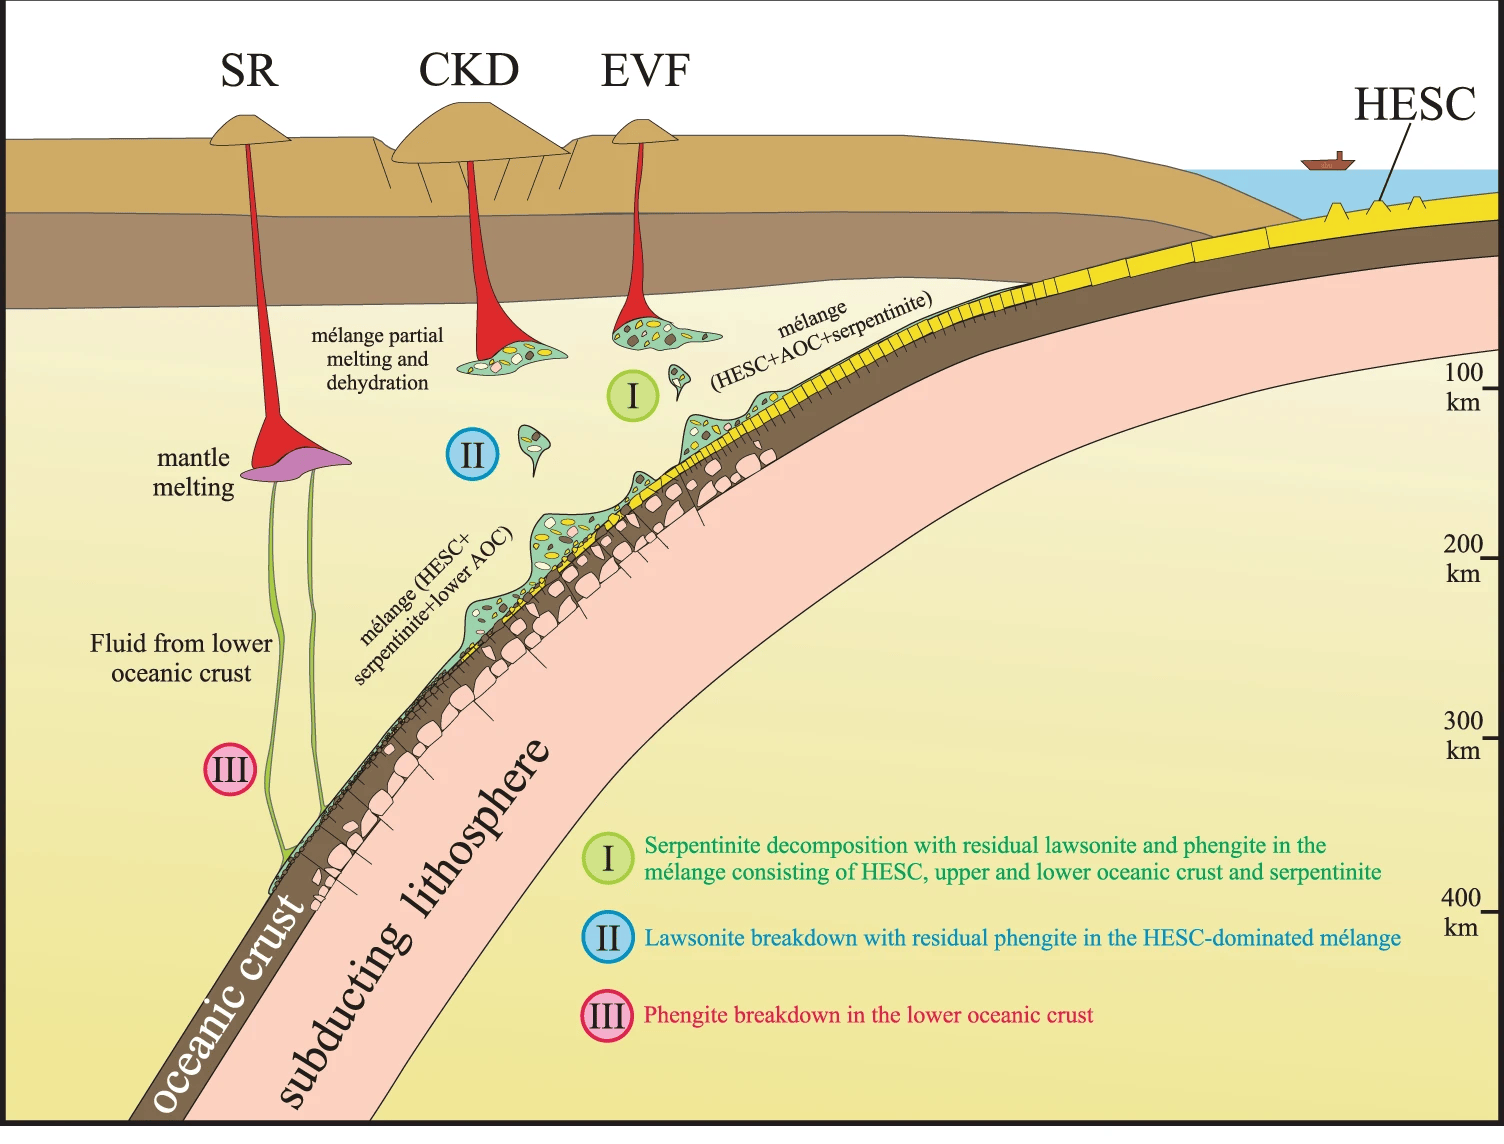
\includegraphics[width=0.7\linewidth]{graphics/subduzione_kamchatka.png}
    \caption{Produzione di magma in Kamchatka causata dalla subduzione della placca del Pacifico, con riferimento ai tre fronti vulcanici della regione: Sredinny Range (SR), Central Kamchatka Depression (CKD) e Eastern Volcanic Front (EVF). In particolare si fa riferimento alla subduzione della catena sottomarina Hawaii-Emperor (Hawaii-Emperor Seamount Chain, HESC). Le informazioni aggiuntive riportate, trascurabili in questo lavoro, sono discusse nel dettaglio nell'articolo di \citet{Shu2022Kamchatka} da cui è stata presa la figura.}
    \label{fig:subduzione_kamchatka}
\end{figure}

Nello specifico, la penisola della Kamchatka è costituita da tre fronti vulcanici (Fig. \ref{fig:Kamchatka_volcano_map}): lo Sredinny Range (SR), l'Eastern Volcanic Front (EVF) e la Central Kamchatka Depression (CKD). Lo SR è il più antico, composto principalmente da rocce granitiche, formatesi principalmente durante due fasi: la prima durante il Campaniano (circa \qty{80}{\Ma}) e la seconda durante l'Eocene (circa \qty{52}{\Ma}) \citep{Luchitskaya2008}. Molto attivo durante l'Oligocene (circa \qty{30}{\Ma}), ad oggi risulta quasi estinto. La CKD si sarebbe formata durante Eocene e Pliocene (circa \qty{5}{\Ma}), come un bacino di avanarco. Bacini di questo tipo rappresentano zone di subsidenza, cioè aree in cui la crosta si abbassa progressivamente, situate tra la fossa oceanica in subduzione (situata sulla placca oceanica in subduzione) e la catena montuosa o l'arco vulcanico della placca sovrastante. La CKD è il risultato di una subduzione più occidentale rispetto alla posizione attuale, avvenuta sotto lo SR, all'epoca fronte vulcanico attivo \citep{mantle_and_crust_sources_Klyuchevskoy}.
Il EVF è invece il fronte più recente, in cui si trovano vulcani più giovani, formatisi durante Pleistocene e Olocene (le due epoche geologiche più recenti), a causa della subduzione tutt'ora presente.


In questa tesi i vulcani presi in esame sono due: il Krasheninnikov e il Klyuchevskoy situati nella CKD. Per entrambi è stata rilevata una ripresa dell'attività eruttiva nei giorni successivi al terremoto del 29 luglio 2025.


\begin{figure}[H]
    \centering
    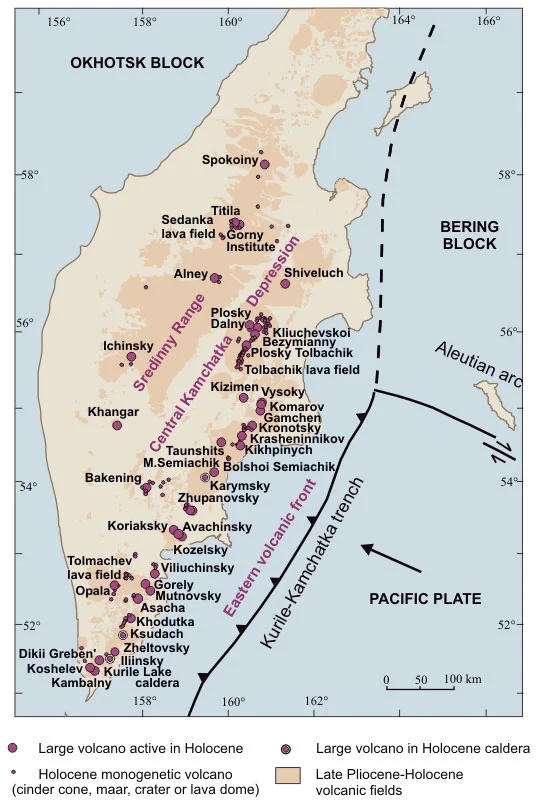
\includegraphics[width=0.7\textwidth]{graphics/kamchatka_volcano_map.png}
    \caption{Mappa di vari vulcani presenti nella penisola della Kamchatka. 
    Le linee nere, continue e tratteggiate, rappresentano i margini tra le placche. 
    La freccia nera disegnata sulla placca del Pacifico rappresenta la direzione in cui questa subduce alla placca di Okhotsk. 
    Lo spostamento dei fronti vulcanici avviene da nord-ovest, dove si trova lo Sredinny Range, verso l'East Volcanic Front nel sud-est della penisola. 
    Tra questi due fronti è presente la Central Kamchatka Depression 
    \citep{Boniecki2019Kamchatka}.}
    \label{fig:Kamchatka_volcano_map}
\end{figure}


\subsection{Klyuchevskoy}
Il Klyuchevskoy (Fig. \ref{fig:photo_klyuchevskoy}) è il vulcano più alto (\qty{4750}{\meter} sul livello del mare) e più attivo della Kamchatka, formatosi circa 6000 anni fa nella regione settentrionale della CKD.
Nonostante sia un vulcano molto giovane è proprio grazie alle frequenti eruzioni che è riuscito a svilupparsi fino a raggiungere l'altezza attuale.
L'edificio vulcanico è a forma di cono e risulta fortemente simmetrico. Ciò è dovuto alla bassa viscosità della lava emessa dalle sue eruzioni, che scorrendo rapidamente ha portato a fianchi regolari in tutte le direzioni.
Il Klyuchevskoy nello specifico è uno stratovulcano, formato cioè da strati alternati di lava e materiale piroclastico (frammenti di roccia vulcanica espulsi durante le eruzioni).
Il magma eruttato dal Klyuchevskoy è di carattere basaltico-andesitico. Il magma basaltico presenta una concentrazione di silicati minore rispetto al magma andesitico e risulta quindi meno viscoso. Un magma di questo tipo è associato ad attività esplosiva sia moderata che violenta.
Si stima che tra il 1930 e il 2005 il vulcano abbia eruttato circa \qty{1.5e9}{\meter\cubed} di lava, con un rate di emissione di circa \qty{0.67}{\meter\cubed\per\second} \citep{coppola_thermal_remote_sensing_2021}.
Come detto, il Klyuchevskoy non ha mai avuto lunghi periodi di inattività. Dati del \citet{GVP_Klyuchevskoy} indicano che il vulcano aveva eruttato già nell'aprile 2025. Il 30 luglio 2025, poco dopo la scossa di terremoto \(\mathrm{M}\,8.8\), è stata osservata una ripresa dell'attività eruttiva.

\begin{figure}[H]
    \centering
    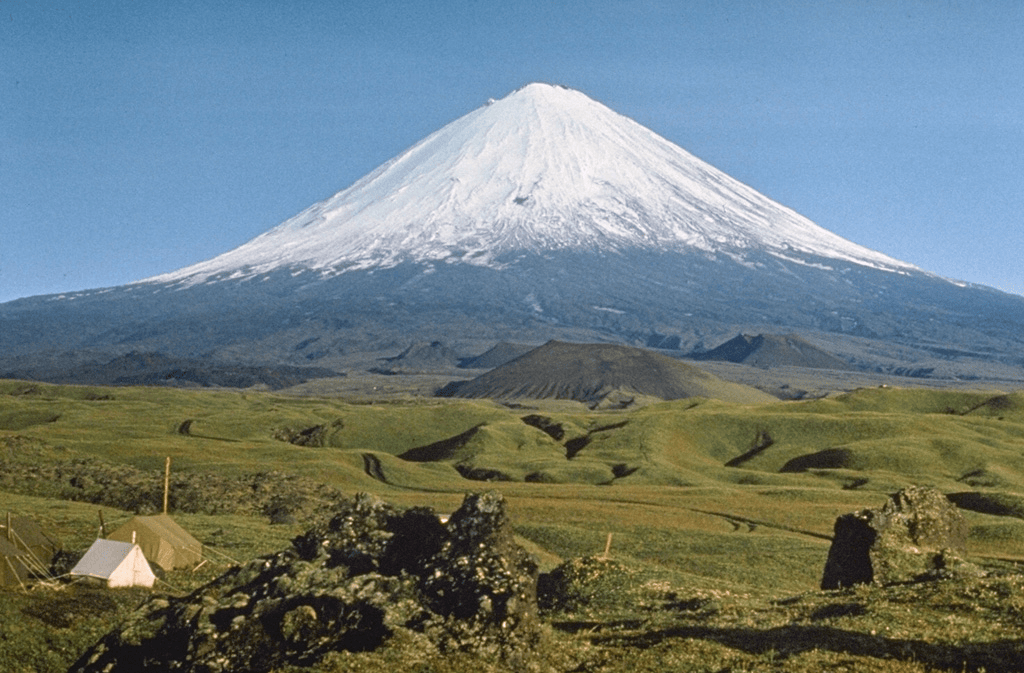
\includegraphics[width=0.75\linewidth]{graphics/photo_klyuchevskoy.png}
    \caption{Vulcano Klyuchevskoy [preso da \citet{GVP_Klyuchevskoy}]}
    \label{fig:photo_klyuchevskoy}
\end{figure}

% \begin{figure}[H]
%     \centering
%     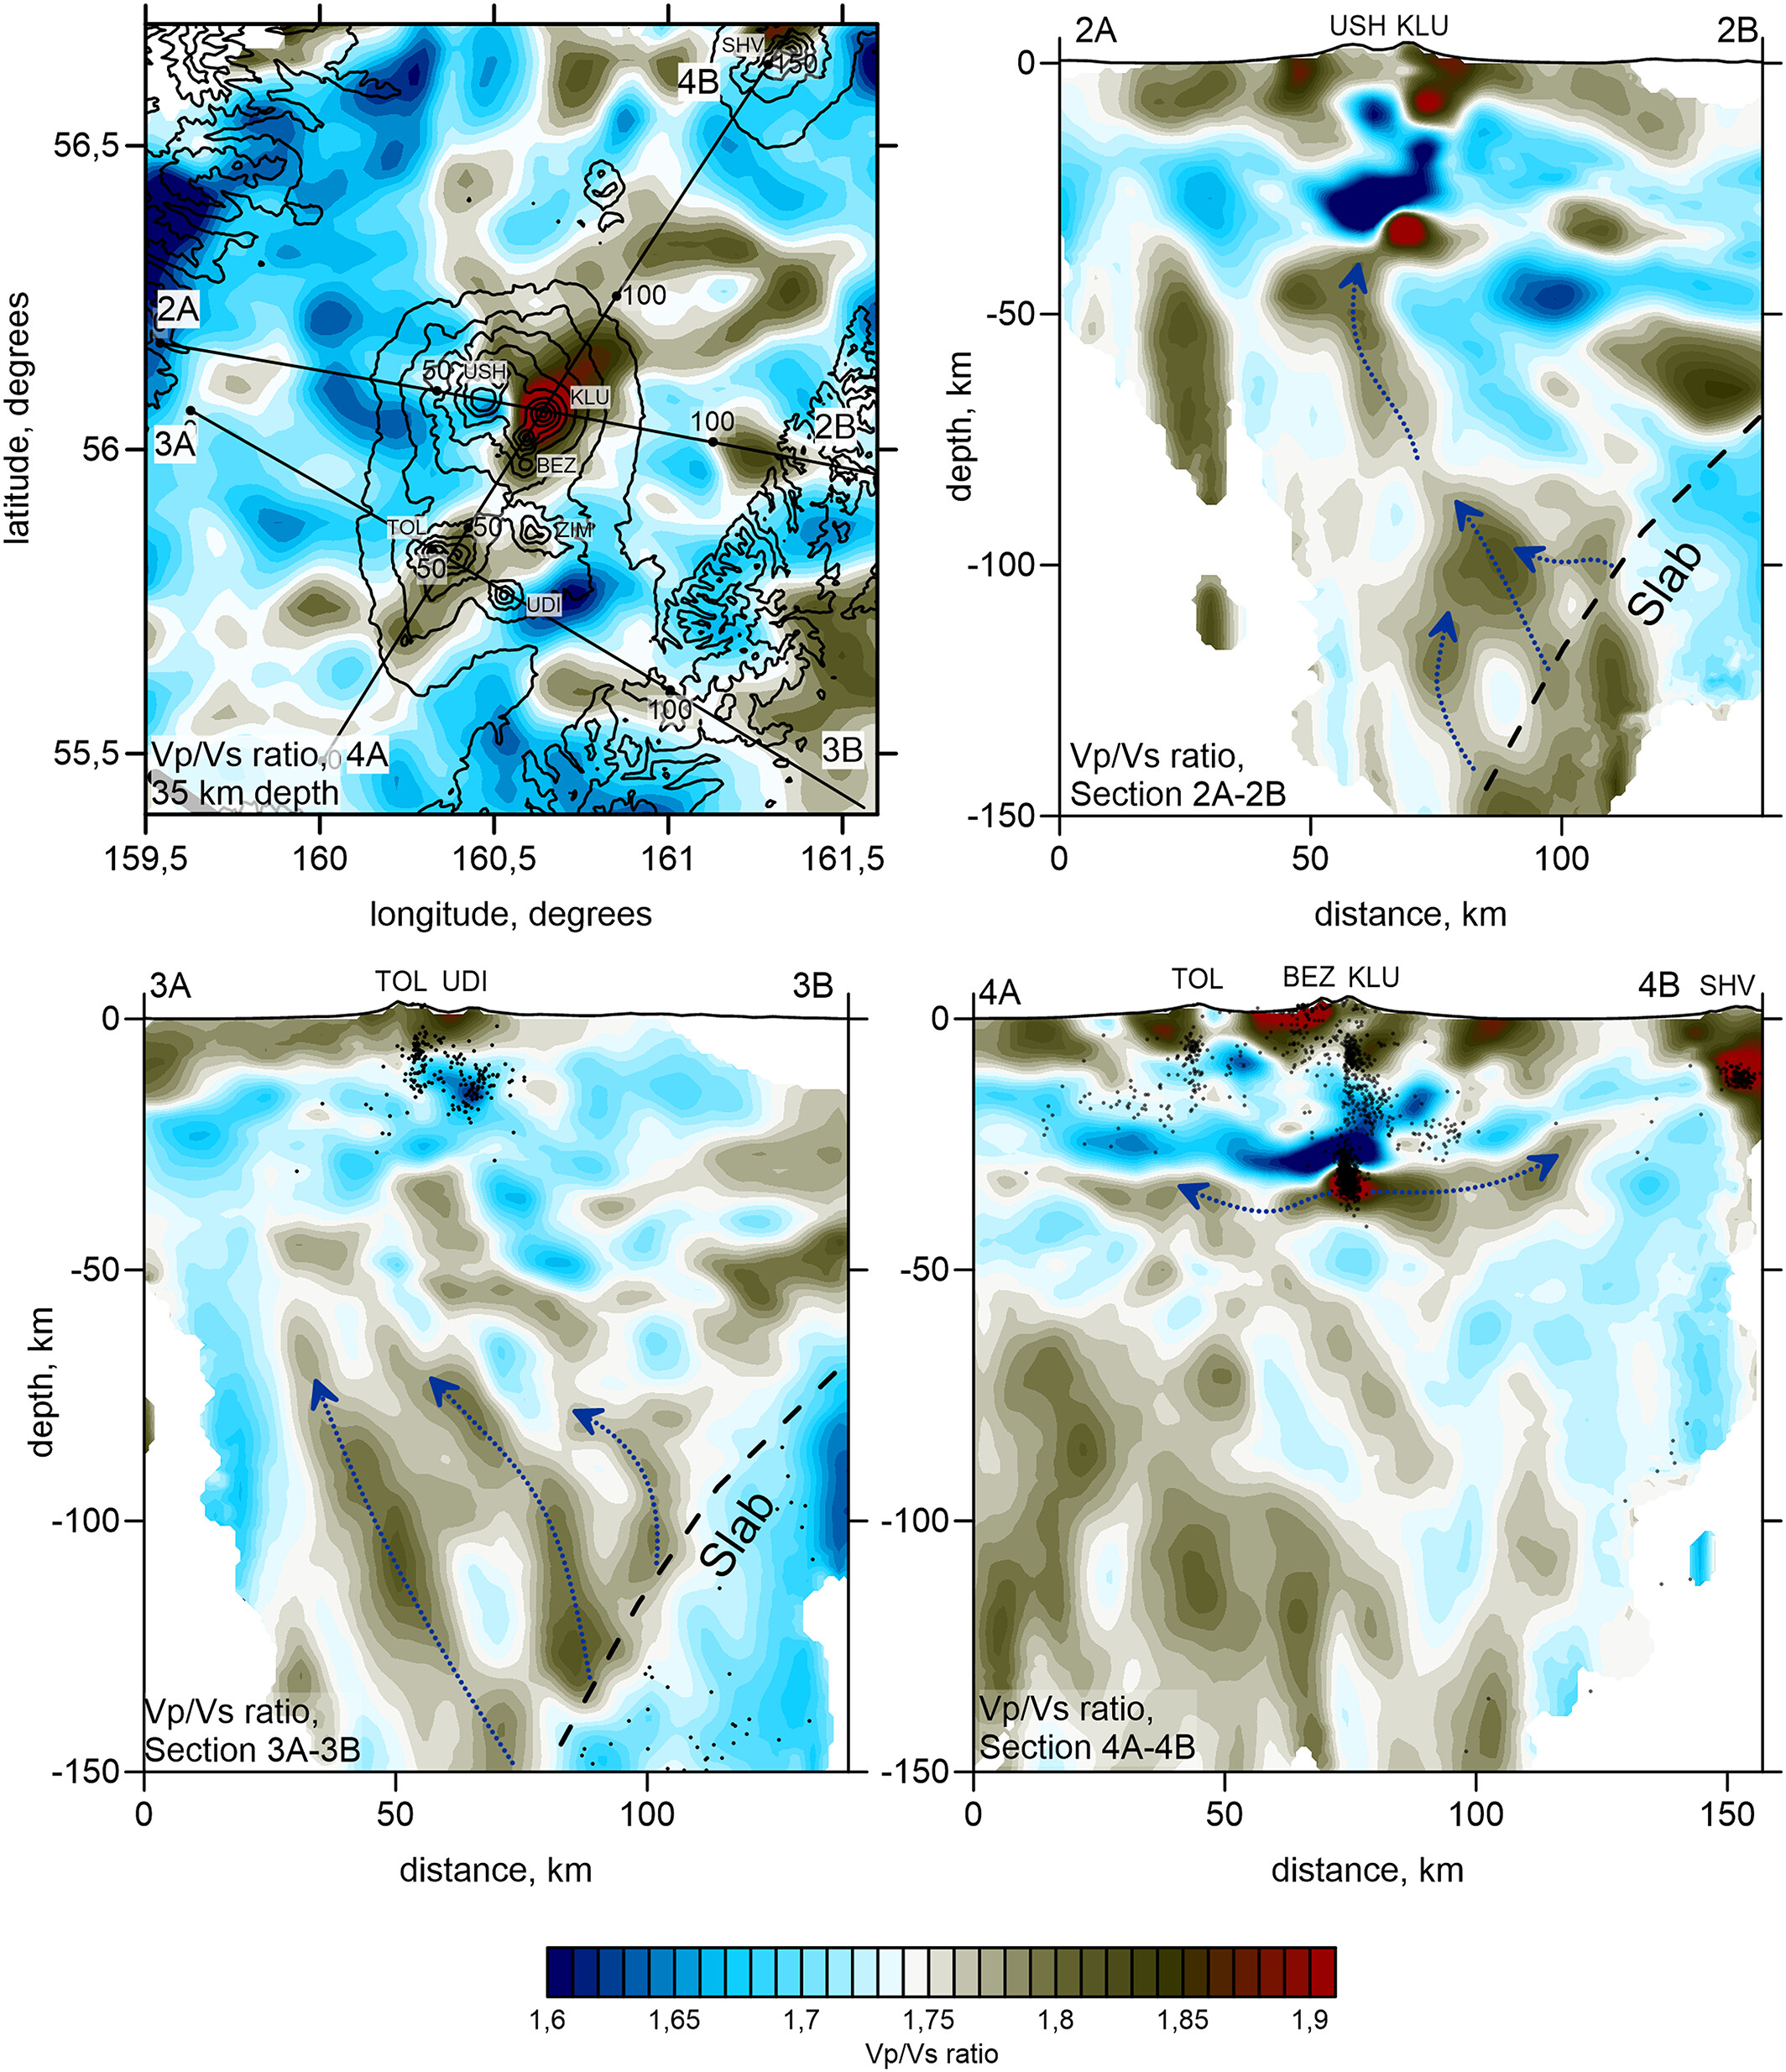
\includegraphics[width=0.75\linewidth]{graphics/mantle_sources_fig14.png}
%     \caption{[preso da \citet{mantle_and_crust_sources_Klyuchevskoy}]}
%     \label{fig:mantle_sources_fig14}
% \end{figure}


\subsection{Krasheninnikov}
Il Krasheninnikov (Fig. \ref{fig:photo_krasheninnikov}) è un vulcano costituito da due stratovulcani sovrapposti all'interno di una caldera formatasi nel Pleistocene, con diametro di \qty{9}{\kilo\meter} e altezza massima di \qty{1816}{\meter}
 \citep{GVP_Krasheninnikov}. Una caldera è una depressione generata a seguito del collasso di un edificio vulcanico sopra la camera magmatica, tipicamente dopo un'eruzione.
Studiando dei depositi piroclastici datati a circa \qty{30}{\ka},
\citet{Ponomareva2025Krasheninnikov} sono riusciti a stimare il volume piroclastico minimo eruttato e la magnitudo dell'eruzione che avrebbe portato al collasso della camera magmatica e alla conseguente formazione della caldera. Il volume è di circa \qty{13}{\kilo\meter\cubed}, mentre la magnitudo è di 6.1.
I due stratovulcani sono situati su una frattura orientata NE-SW.
La formazione dell'edificio a sud
è iniziata circa \qty{11}{\ka}, mentre quella dell'edificio a nord circa 6500 anni fa.
Prima del terremoto del 29 luglio 2025, l'ultima attività vulcanica del Krasheninnikov è datata attorno all'anno 1550. L'eruzione ha coinvolto entrambi gli edifici all'interno della caldera, con un emissione di lava da una bocca del fianco sud-ovest del cono meridionale e con la formazione di un nuovo cratere sulla cima del cono settentrionale \citep{GVP_Krasheninnikov}.
In data 2 agosto 2025, è stata registrata un'eruzione di tipo esplosivo, a circa \qty{1650}{\meter}. Le cenerei prodotte si sono alzate di \qty{3}{}-\qty{4}{\kilo\meter} rispetto alla cime dell'edificio a nord \citep{GVP_Krasheninnikov}. Inoltre, si è verificata un'eruzione effusiva, prodotta a seguito dell'apertura di una bocca sul fianco nord-ovest dell'edificio.

\begin{figure}[H]
    \centering
    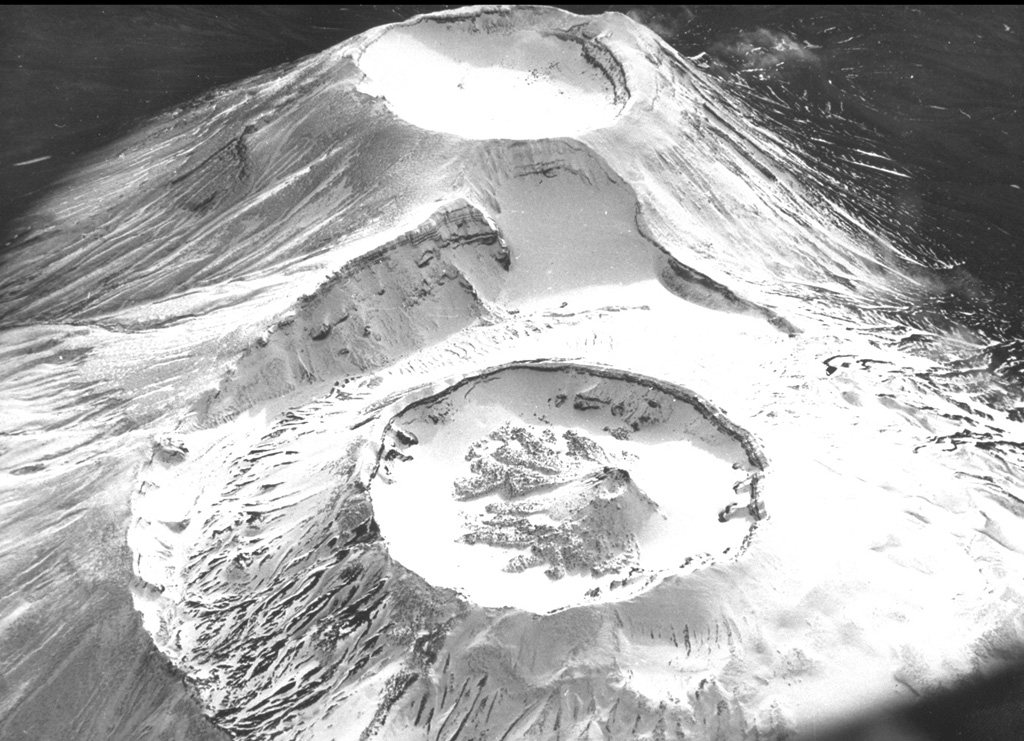
\includegraphics[width=0.7\linewidth]{graphics/photo_krasheninnikov.png}
    \caption{Vulcano Krasheninnikov [preso da \citet{GVP_Krasheninnikov}]}
    \label{fig:photo_krasheninnikov}
\end{figure}